\documentclass[journal,12pt,twocolumn]{IEEEtran}
%
\usepackage{setspace}
\usepackage{textcomp}
\usepackage{gensymb}
%\doublespacing
\singlespacing

\usepackage[cmex10]{amsmath}
\usepackage{amsthm}
%\usepackage{iithtlc}
\usepackage{mathrsfs}
\usepackage{txfonts}
\usepackage{stfloats}
\usepackage{bm}
\usepackage{cite}
\usepackage{cases}
\usepackage{subfig}
%\usepackage{xtab}
\usepackage{longtable}
\usepackage{multirow}
%\usepackage{algorithm}
%\usepackage{algpseudocode}
\usepackage{enumitem}
\usepackage{mathtools}
\usepackage{steinmetz}
\usepackage{tikz}
\usepackage{circuitikz}
\usepackage{verbatim}
\usepackage{tfrupee}
\usepackage[breaklinks=true]{hyperref}
%\usepackage{stmaryrd}
\usepackage{tkz-euclide} % loads  TikZ and tkz-base
%\usetkzobj{all}
\usetikzlibrary{calc,math}
\usepackage{listings}
    \usepackage{color}                                            %%
    \usepackage{array}                                            %%
    \usepackage{longtable}                                        %%
    \usepackage{calc}                                             %%
    \usepackage{multirow}                                         %%
    \usepackage{hhline}                                           %%
    \usepackage{ifthen}                                           %%
  %optionally (for landscape tables embedded in another document): %%
    \usepackage{lscape}     
\usepackage{multicol}
\usepackage{chngcntr}
%\usepackage{enumerate}

%\usepackage{wasysym}
%\newcounter{MYtempeqncnt}
\DeclareMathOperator*{\Res}{Res}
%\renewcommand{\baselinestretch}{2}
\renewcommand\thesection{\arabic{section}}
\renewcommand\thesubsection{\thesection.\arabic{subsection}}
\renewcommand\thesubsubsection{\thesubsection.\arabic{subsubsection}}

\renewcommand\thesectiondis{\arabic{section}}
\renewcommand\thesubsectiondis{\thesectiondis.\arabic{subsection}}
\renewcommand\thesubsubsectiondis{\thesubsectiondis.\arabic{subsubsection}}

% correct bad hyphenation here
\hyphenation{op-tical net-works semi-conduc-tor}
\def\inputGnumericTable{}                                 %%

\lstset{
%language=C,
frame=single, 
breaklines=true,
columns=fullflexible
}
\newenvironment{amatrix}[1]{%
  \left(\begin{array}{@{}*{#1}{c}|c@{}}
}{%
  \end{array}\right)
}
\DeclarePairedDelimiter\abs{\lvert}{\rvert}%
\DeclarePairedDelimiter\norm{\lVert}{\rVert}%

% Swap the definition of \abs* and \norm*, so that \abs
% and \norm resizes the size of the brackets, and the 
% starred version does not.
\makeatletter
\let\oldabs\abs
\def\abs{\@ifstar{\oldabs}{\oldabs*}}
%
\let\oldnorm\norm
\def\norm{\@ifstar{\oldnorm}{\oldnorm*}}
\makeatother

\newtheorem{theorem}{Theorem}[section]
\newtheorem{problem}{Problem}
\newtheorem{proposition}{Proposition}[section]
\newtheorem{lemma}{Lemma}[section]
\newtheorem{corollary}[theorem]{Corollary}
\newtheorem{example}{Example}[section]
\newtheorem{definition}[problem]{Definition}
%\newtheorem{thm}{Theorem}[section] 
%\newtheorem{defn}[thm]{Definition}
%\newtheorem{algorithm}{Algorithm}[section]
%\newtheorem{cor}{Corollary}
\newcommand{\BEQA}{\begin{eqnarray}}
\newcommand{\EEQA}{\end{eqnarray}}
\newcommand{\define}{\stackrel{\triangle}{=}}
\bibliographystyle{IEEEtran}
%\bibliographystyle{ieeetr}
\providecommand{\mbf}{\mathbf}
\providecommand{\pr}[1]{\ensuremath{\Pr\left(#1\right)}}
\providecommand{\qfunc}[1]{\ensuremath{Q\left(#1\right)}}
\providecommand{\sbrak}[1]{\ensuremath{{}\left[#1\right]}}
\providecommand{\lsbrak}[1]{\ensuremath{{}\left[#1\right.}}
\providecommand{\rsbrak}[1]{\ensuremath{{}\left.#1\right]}}
\providecommand{\brak}[1]{\ensuremath{\left(#1\right)}}
\providecommand{\lbrak}[1]{\ensuremath{\left(#1\right.}}
\providecommand{\rbrak}[1]{\ensuremath{\left.#1\right)}}
\providecommand{\cbrak}[1]{\ensuremath{\left\{#1\right\}}}
\providecommand{\lcbrak}[1]{\ensuremath{\left\{#1\right.}}
\providecommand{\rcbrak}[1]{\ensuremath{\left.#1\right\}}}
\providecommand{\system}{\overset{\mathcal{H}}{ \longleftrightarrow}}
	%\newcommand{\solution}[2]{\textbf{Solution:}{#1}}
\newcommand{\solution}{\noindent \textbf{Solution: }}
\newcommand{\cosec}{\,\text{cosec}\,}
\providecommand{\dec}[2]{\ensuremath{\overset{#1}{\underset{#2}{\gtrless}}}}
\newcommand{\myvec}[1]{\ensuremath{\begin{pmatrix}#1\end{pmatrix}}}
\newcommand{\mydet}[1]{\ensuremath{\begin{vmatrix}#1\end{vmatrix}}}
%\numberwithin{equation}{section}
\numberwithin{equation}{subsection}
%\numberwithin{problem}{section}
%\numberwithin{definition}{section}
\makeatletter
\@addtoreset{figure}{problem}
\makeatother
\let\StandardTheFigure\thefigure
\let\vec\mathbf
\usepackage{mathtools, nccmath}
\begin{document}
\begin{center}
\huge Assignment 5\\
\large SUBHASISH SAIKIA\\
\large AI20MTECH14001\\
\end{center}
\vspace{0.5cm}
\begin{abstract}
This document explains the properties of tangent to a  circle and how to find the  equation of the tangent to the circle at a given point. 
\end{abstract}
\vspace{0.5cm}
Download all python codes from 
\begin{lstlisting}
https://github.com/subhasishsaikia22/EE5609-Matrix-theory
\end{lstlisting}
%
and latex-tikz codes from 
\begin{lstlisting}
https://github.com/subhasishsaikia22/EE5609-Matrix-theory
\end{lstlisting}
%
\vspace{0.5cm}
\section{Problem}
Find the equation of the tangent to the following
curve at the points stated:
\begin{align}
    \vec{x^Tx}=25,\myvec{3\\4}
\end{align}

\section{Explanation}
The given equation of the curve:
\begin{align}
    \vec{x^Tx}=25\label{giveneqn}
\end{align}
The general equation of a second degree can
be expressed as:
\begin{align}
    \vec{x^TVx}+2\vec{u^Tx}+f=0 \label{geneqn}
\end{align}
Comparing \eqref{geneqn} with \eqref{giveneqn}:\\
\begin{align}
    \vec{V} =  \vec{I},\vec{u}=\myvec{0\\0} and f=-25 
\end{align}
For $\vec{V}$ =  $\vec{I}$, \eqref{geneqn} represents a circle. \quad$\vec{c}$ represent the center , r the radius  and $\vec{q}$ the point of contact of the tangent to the circle .\\
The center and radius is given by:
\begin{align}
\vec{c}=-\vec{u}=\myvec{0\\0}\label{ceneqn}\\
r=\sqrt{\vec{u^Tu}-f}=\sqrt{0-(-25)}=5
\end{align}

The given point of contact
\begin{align}
 \vec{q}=\myvec{3\\4} \label{coord}  
\end{align}
The direction vector of the line joining the point $\vec{q}$ and the center $\vec{c}$ is:
\begin{align}
 \vec{n}= \vec{q}-\vec{c}\\
  \Longrightarrow\vec{n}= \vec{q}+\vec{u}=\myvec{3\\4}
\end{align}
The vector $\vec{n}$ is  normal to the tangent of the circle, drawn at $\vec{q}$\\
The equation of the tangent is
\begin{align}
 \vec{n^T}\myvec{\vec{x}-\vec{q}}=0\\
 \vec{n^T}\vec{x}=c\\
 \end{align}
 where 
 \begin{align}
c=\vec{n^T}\vec{q}\\
  \Longrightarrow c=\myvec{3\quad4}\myvec{3 \\4}=25
 \end{align}
Thus the equation of the tangent to the curve at $\vec{q}$ is
\begin{align}
    \vec{n^T}\vec{x}=25\\
     \Longrightarrow \myvec{3\quad4}\vec{x}=25
\end{align}

\begin{figure}[!]
 \begin{center}
  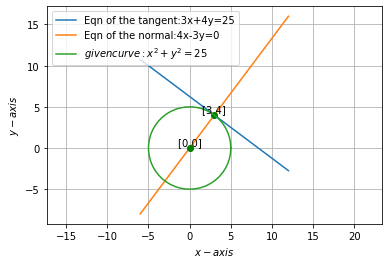
\includegraphics[width=\columnwidth]{assignment5_fig.png}
    \caption{This is the 2D diagram of the given curve  $\vec{x^Tx}=25$ and the tangent to it at $\myvec{3\\4}$}
    \label{myfig:1}
    \end{center}
\end{figure}
\end{document}
